\documentclass[12pt,addpoints]{repaso}
\grado{3}
\nivel{Secundaria}
\cicloescolar{2023-2024}
\materia{Matemáticas \color{darkgray}\small con adecuación curricular}
\unidad{3}
\title{Practica la Unidad}
\aprendizajes{
    \item Representa con diferentes expresiones aditivas (suma y resta) cantidades menores a 1000.
    \item Representa, con apoyo de material concreto y modelos gráficos, fracciones: medios, cuartos, octavos, dieciseisavos, para expresar el resultado de mediciones y repartos en situaciones vinculadas a su contexto.
    \item Resuelve multiplicaciones cuyo producto es un mero natural de tres cifras.
    \item Resuelve divisiones con divisor de una cifra. 
    }
\author{Melchor Pinto, J.C.}
\begin{document}
\INFO
\begin{questions}
    \questionboxed[10]{Realiza las siguientes sumas:

        \begin{multicols}{5}
            \begin{parts}
                \part \ifprintanswers{\large  \quad   \opadd[hfactor=decimal,resultstyle=\color{red},carryadd=true,carrysub=false]{475}{39} \\[1ex]}
                \else{          \large  \quad  \opadd[hfactor=decimal,resultstyle=\color{red},carryadd=true,carrysub=false]{475}{39} \\[1ex]}
                \fi

                \part \ifprintanswers{\large  \quad  \opadd[hfactor=decimal,resultstyle=\color{red},carrysub=true]{463}{229} \\[1ex]}
                \else{          \large  \quad  \opadd[hfactor=decimal,resultstyle=\color{red},carryadd=true,carrysub=false]{463}{229} \\[1ex]}
                \fi

                \part \ifprintanswers{\large  \quad  \opadd[hfactor=decimal,resultstyle=\color{red},carrysub=true]{375}{316} \\[1ex]}
                \else{          \large  \quad  \opadd[hfactor=decimal,resultstyle=\color{red},carryadd=true,carrysub=false]{375}{316} \\[1ex]}
                \fi

                \part \ifprintanswers{\large  \quad  \opadd[hfactor=decimal,resultstyle=\color{red},carrysub=true]{397}{19} \\[1ex]}
                \else{          \large  \quad  \opadd[hfactor=decimal,resultstyle=\color{red},carryadd=true,carrysub=false]{397}{19} \\[1ex]}
                \fi

                \part \ifprintanswers{\large  \quad  \opadd[hfactor=decimal,resultstyle=\color{red},carrysub=true]{468}{192} \\[1ex]}
                \else{          \large  \quad  \opadd[hfactor=decimal,resultstyle=\color{red},carryadd=true,carrysub=false]{468}{192} \\[1ex]}
                \fi

                \part \ifprintanswers{\large  \quad  \opadd[hfactor=decimal,resultstyle=\color{red},carrysub=true]{472}{356} \\[1ex]}
                \else{          \large  \quad  \opadd[hfactor=decimal,resultstyle=\color{red},carryadd=true,carrysub=false]{472}{356} \\[1ex]}
                \fi

                \part \ifprintanswers{\large  \quad  \opadd[hfactor=decimal,resultstyle=\color{red},carrysub=true]{461}{312} \\[1ex]}
                \else{          \large  \quad  \opadd[hfactor=decimal,resultstyle=\color{red},carryadd=true,carrysub=false]{461}{312} \\[1ex]}
                \fi

                \part \ifprintanswers{\large  \quad  \opadd[hfactor=decimal,resultstyle=\color{red},carrysub=true]{523}{408} \\[1ex]}
                \else{          \large  \quad  \opadd[hfactor=decimal,resultstyle=\color{red},carryadd=true,carrysub=false]{523}{408} \\[1ex]}
                \fi

                \part \ifprintanswers{\large  \quad  \opadd[hfactor=decimal,resultstyle=\color{red},carrysub=true]{478}{229} \\[1ex]}
                \else{          \large  \quad  \opadd[hfactor=decimal,resultstyle=\color{red},carryadd=true,carrysub=false]{478}{229} \\[1ex]}
                \fi

                \part \ifprintanswers{\large  \quad  \opadd[hfactor=decimal,resultstyle=\color{red},carrysub=true]{442}{261} \\[1ex]}
                \else{          \large  \quad  \opadd[hfactor=decimal,resultstyle=\color{red},carryadd=true,carrysub=false]{442}{261} \\[1ex]}
                \fi
            \end{parts}
        \end{multicols}
    }

    \questionboxed[10]{Realiza las siguientes restas:

        \begin{multicols}{5}
            \begin{parts}
                \part \ifprintanswers{\large  \quad  \opsub[hfactor=decimal,resultstyle=\color{red},carrysub=true]{475}{39} \\[1ex]}
                \else{          \large  \quad  \opsub[hfactor=decimal,resultstyle=\color{white},carrysub=false]{475}{39} \\[1ex]}
                \fi

                \part \ifprintanswers{\large  \quad  \opsub[hfactor=decimal,resultstyle=\color{red},carrysub=true]{463}{229} \\[1ex]}
                \else{          \large  \quad  \opsub[hfactor=decimal,resultstyle=\color{white},carrysub=false]{463}{229} \\[1ex]}
                \fi

                \part \ifprintanswers{\large  \quad  \opsub[hfactor=decimal,resultstyle=\color{red},carrysub=true]{375}{316} \\[1ex]}
                \else{          \large  \quad  \opsub[hfactor=decimal,resultstyle=\color{white},carrysub=false]{375}{316} \\[1ex]}
                \fi

                \part \ifprintanswers{\large  \quad  \opsub[hfactor=decimal,resultstyle=\color{red},carrysub=true]{397}{19} \\[1ex]}
                \else{          \large  \quad  \opsub[hfactor=decimal,resultstyle=\color{white},carrysub=false]{397}{19} \\[1ex]}
                \fi

                \part \ifprintanswers{\large  \quad  \opsub[hfactor=decimal,resultstyle=\color{red},carrysub=true]{468}{192} \\[1ex]}
                \else{          \large  \quad  \opsub[hfactor=decimal,resultstyle=\color{white},carrysub=false]{468}{192} \\[1ex]}
                \fi

                \part \ifprintanswers{\large  \quad  \opsub[hfactor=decimal,resultstyle=\color{red},carrysub=true]{472}{356} \\[1ex]}
                \else{          \large  \quad  \opsub[hfactor=decimal,resultstyle=\color{white},carrysub=false]{472}{356} \\[1ex]}
                \fi

                \part \ifprintanswers{\large  \quad  \opsub[hfactor=decimal,resultstyle=\color{red},carrysub=true]{461}{312} \\[1ex]}
                \else{          \large  \quad  \opsub[hfactor=decimal,resultstyle=\color{white},carrysub=false]{461}{312} \\[1ex]}
                \fi

                \part \ifprintanswers{\large  \quad  \opsub[hfactor=decimal,resultstyle=\color{red},carrysub=true]{523}{408} \\[1ex]}
                \else{          \large  \quad  \opsub[hfactor=decimal,resultstyle=\color{white},carrysub=false]{523}{408} \\[1ex]}
                \fi

                \part \ifprintanswers{\large  \quad  \opsub[hfactor=decimal,resultstyle=\color{red},carrysub=true]{478}{229} \\[1ex]}
                \else{          \large  \quad  \opsub[hfactor=decimal,resultstyle=\color{white},carrysub=false]{478}{229} \\[1ex]}
                \fi

                \part \ifprintanswers{\large  \quad  \opsub[hfactor=decimal,resultstyle=\color{red},carrysub=true]{442}{261} \\[1ex]}
                \else{          \large  \quad  \opsub[hfactor=decimal,resultstyle=\color{white},carrysub=false]{442}{261} \\[1ex]}
                \fi
            \end{parts}
        \end{multicols}
    }

    \questionboxed[10]{Realiza las siguientes multiplicaciones:

        \begin{multicols}{5}
            \begin{parts}
                \part \ifprintanswers{\large \quad \opmul[hfactor=decimal,resultstyle=\color{red},displayintermediary=None]{256}{3} \\[4em]}
                \else{          \large \quad \opmul[hfactor=decimal,resultstyle=\color{white},displayintermediary=None]{256}{3} \\[4em]}
                \fi

                \part \ifprintanswers{\large \quad \opmul[hfactor=decimal,resultstyle=\color{red},displayintermediary=None]{342}{8} \\[4em]}
                \else{          \large \quad \opmul[hfactor=decimal,resultstyle=\color{white},displayintermediary=None]{342}{8} \\[4em]}
                \fi

                \part \ifprintanswers{\large \quad \opmul[hfactor=decimal,resultstyle=\color{red},displayintermediary=None]{241}{8} \\[4em]}
                \else{          \large \quad \opmul[hfactor=decimal,resultstyle=\color{white},displayintermediary=None]{241}{8} \\[4em]}
                \fi

                \part \ifprintanswers{\large \quad \opmul[hfactor=decimal,resultstyle=\color{red},displayintermediary=None]{3927}{6} \\[4em]}
                \else{          \large \quad \opmul[hfactor=decimal,resultstyle=\color{white},displayintermediary=None]{3927}{6} \\[4em]}
                \fi

                \part \ifprintanswers{\large \quad \opmul[hfactor=decimal,resultstyle=\color{red},displayintermediary=None]{1333}{4} \\[4em]}
                \else{          \large \quad \opmul[hfactor=decimal,resultstyle=\color{white},displayintermediary=None]{1333}{4} \\[4em]}
                \fi

                \part \ifprintanswers{\large \quad \opmul[hfactor=decimal,resultstyle=\color{red},displayintermediary=None]{1901}{8} \\[4em]}
                \else{          \large \quad \opmul[hfactor=decimal,resultstyle=\color{white},displayintermediary=None]{1901}{8} \\[4em]}
                \fi
                \part \ifprintanswers{ \quad \opmul[hfactor=decimal,resultstyle=\color{red},displayintermediary=all]{19}{19} \\[4em]}
                \else{          \large \quad \opmul[hfactor=decimal,resultstyle=\color{white},displayintermediary=None]{19}{19} \\[4em]}
                \fi

                \part \ifprintanswers{ \quad \opmul[hfactor=decimal,resultstyle=\color{red},displayintermediary=all]{25}{25} \\[4em]}
                \else{          \large \quad \opmul[hfactor=decimal,resultstyle=\color{white},displayintermediary=None]{25}{125} \\[4em]}
                \fi

                \part \ifprintanswers{ \quad \opmul[hfactor=decimal,resultstyle=\color{red},displayintermediary=all]{18}{18} \\[4em]}
                \else{          \large \quad \opmul[hfactor=decimal,resultstyle=\color{white},displayintermediary=None]{18}{18} \\[4em]}
                \fi


                \part \ifprintanswers{ \quad \opmul[hfactor=decimal,resultstyle=\color{red},displayintermediary=all]{17}{17} \\[4em]}
                \else{          \large \quad \opmul[hfactor=decimal,resultstyle=\color{white},displayintermediary=None]{17}{17} \\[4em]}
                \fi
            \end{parts}
        \end{multicols}
    }

    \questionboxed[10]{Realiza las siguientes divisiones:

        \begin{multicols}{5}
            \begin{parts}
                \part \ifprintanswers{\large\opdiv[period,style=text,hrulewidth=0.2pt,vruleperiod=0.7,hfactor=decimal,resultstyle=\color{red}]{123}{6}}
                \else{          \large  \quad $6 \overline{) \ 123\ }$}
                \fi
            \end{parts}
        \end{multicols}
    }

    \questionboxed[10]{Escribe la fracción que representa cada una de las siguientes imágenes:

        \begin{multicols}{3}
            \begin{parts}
                \part \fracquestion{$\dfrac{3}{4}$}{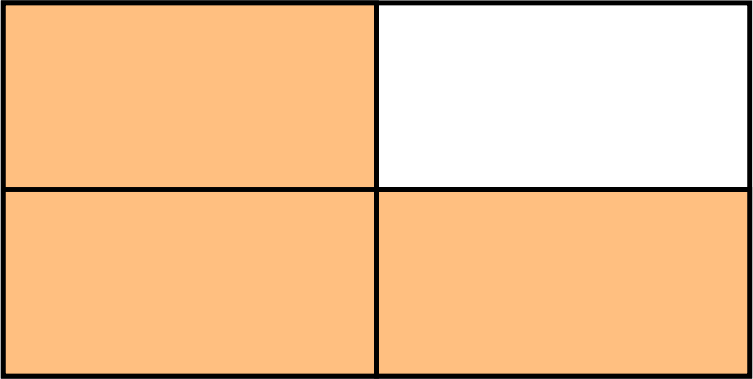
\includegraphics[width=\linewidth]{imagen_frac13.png}}
                \part \fracquestion{$\dfrac{3}{16}$}{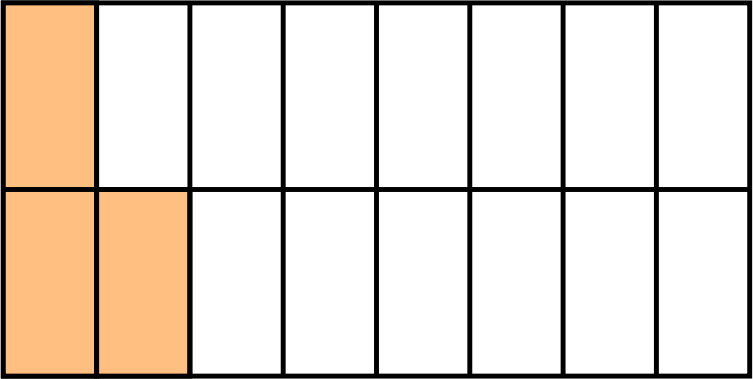
\includegraphics[width=\linewidth]{imagen_frac12.png}}
                \part \fracquestion{$\dfrac{2}{8}$}{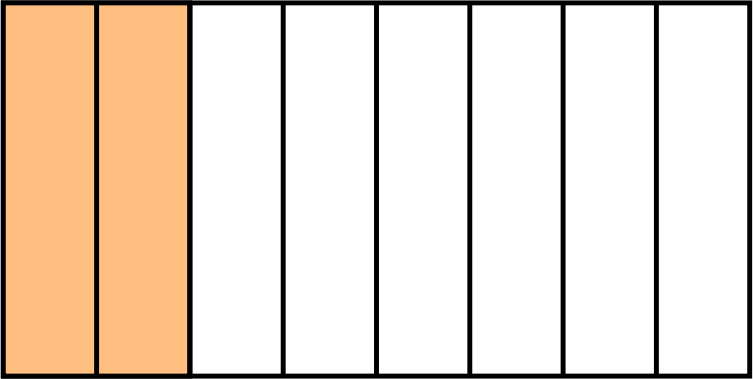
\includegraphics[width=\linewidth]{imagen_frac14.png}}
                \part \fracquestion{$\dfrac{1}{4}$}{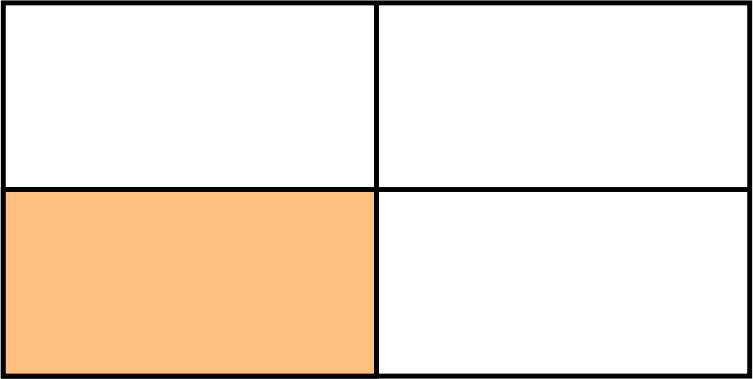
\includegraphics[width=\linewidth]{imagen_frac15.png}}
                \part \fracquestion{$\dfrac{5}{8}$}{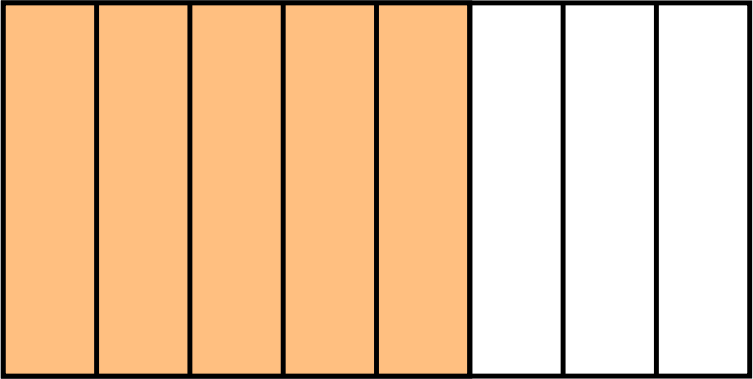
\includegraphics[width=\linewidth]{imagen_frac16.png}}
                \part \fracquestion{$\dfrac{7}{8}$}{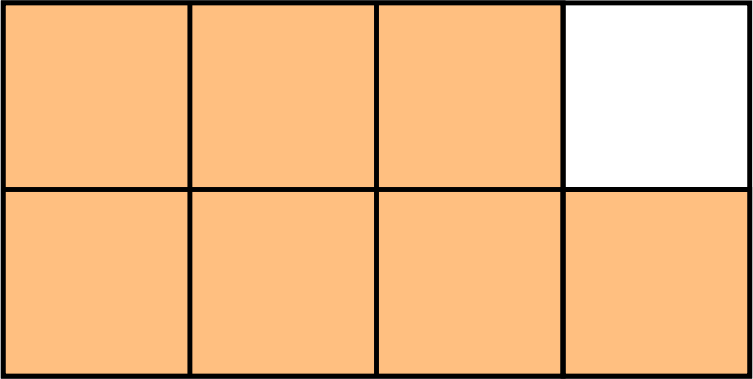
\includegraphics[width=\linewidth]{imagen_frac17.png}}
                \part \fracquestion{$\dfrac{7}{8}$}{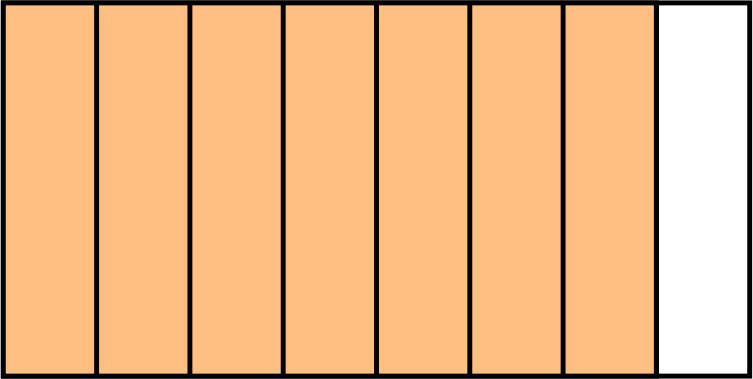
\includegraphics[width=\linewidth]{imagen_frac18.png}}
                \part \fracquestion{$\dfrac{8}{16}$}{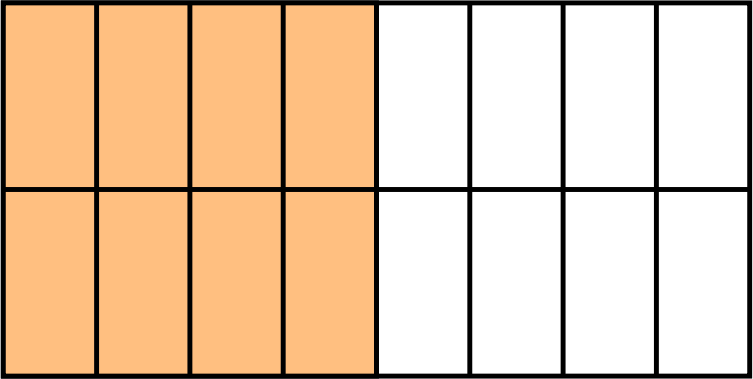
\includegraphics[width=\linewidth]{imagen_frac19.png}}
                \part \fracquestion{$\dfrac{3}{8}$}{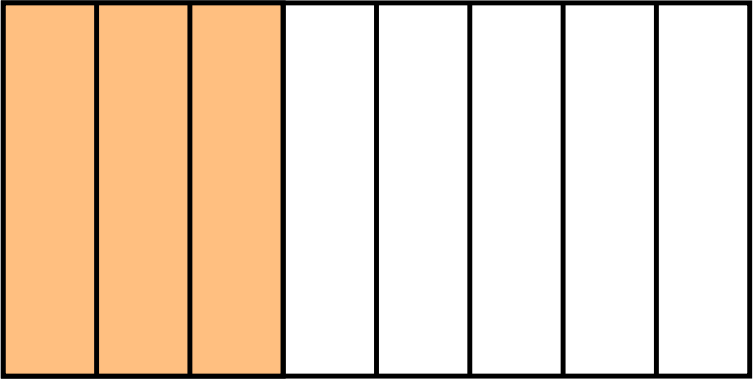
\includegraphics[width=\linewidth]{imagen_frac20.png}}
                \part \fracquestion{$\dfrac{2}{10}$}{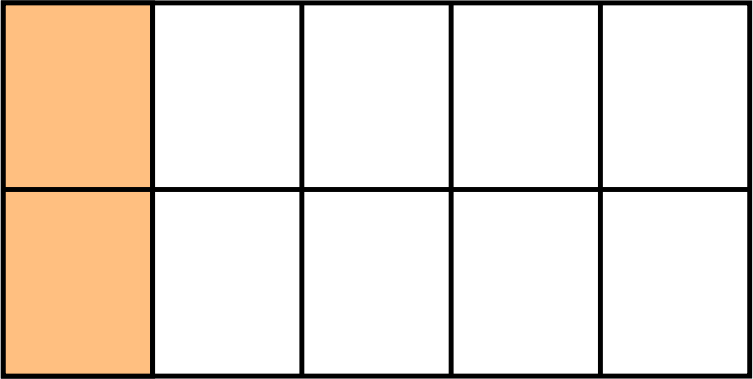
\includegraphics[width=\linewidth]{imagen_frac21.png}}
                \part \fracquestion{$\dfrac{1}{16}$}{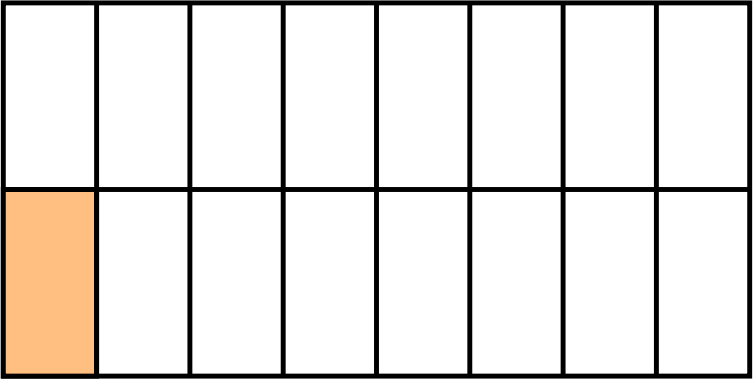
\includegraphics[width=\linewidth]{imagen_frac22.png}}
                \part \fracquestion{$\dfrac{2}{8}$}{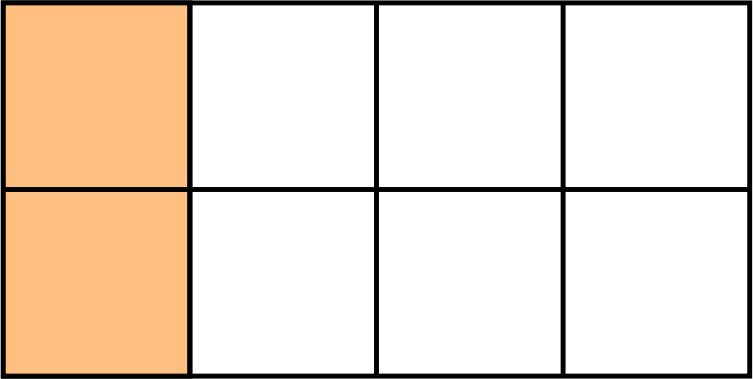
\includegraphics[width=\linewidth]{imagen_frac23.png}}
            \end{parts}
        \end{multicols}
    }

    \questionboxed[10]{Escribe numéricamente la fracción indicada en cada inciso:

        \begin{multicols}{4}
            \begin{parts}
                \part \fracquestion{$\dfrac{5}{8}$}{cinco octavos}
                \part \fracquestion{$\dfrac{7}{9}$}{siete novenos}
                \part \fracquestion{$\dfrac{2}{7}$}{dos séptimos}
                \part \fracquestion{$\dfrac{1}{4}$}{un cuarto}
                \part \fracquestion{$\dfrac{4}{5}$}{cuatro quintos}
                \part \fracquestion{$\dfrac{3}{7}$}{tres séptimos}
                \part \fracquestion{$\dfrac{1}{8}$}{un octavo}
                \part \fracquestion{$\dfrac{2}{3}$}{dos tercios}
                \part \fracquestion{$\dfrac{6}{9}$}{seis novenos}
                \part \fracquestion{$\dfrac{5}{4}$}{cinco cuartos}
                \part \fracquestion{$\dfrac{4}{5}$}{cuatro quintos}
                \part \fracquestion{$\dfrac{9}{6}$}{nueve sextos}
            \end{parts}
        \end{multicols}
    }

    \questionboxed[10]{Realiza las siguientes sumas de fracciones con el mismo denominador:

        \begin{multicols}{5}
            \begin{parts}
                \part \large$\dfrac{2}{2}+\dfrac{2}{2}=$ \fillin[$\dfrac{4}{2}$][0in]
                \part \large$\dfrac{5}{5}+\dfrac{5}{5}=$ \fillin[$\dfrac{10}{5}$][0in]
                \part \large$\dfrac{33}{6}+\dfrac{21}{6}=$ \fillin[$\dfrac{54}{6}$][0in]
                \part \large$\dfrac{1}{9}+\dfrac{7}{9}=$ \fillin[$\dfrac{8}{9}$][0in]
                \part \large$\dfrac{14}{3}+\dfrac{8}{3}=$ \fillin[$\dfrac{22}{3}$][0in]
                \part \large$\dfrac{19}{7}+\dfrac{4}{7}=$ \fillin[$\dfrac{23}{7}$][0in]
                \part \large$\dfrac{13}{6}+\dfrac{10}{6}=$ \fillin[$\dfrac{23}{6}$][0in]
                \part \large$\dfrac{21}{4}+\dfrac{5}{4}=$ \fillin[$\dfrac{26}{4}$][0in]
                \part \large$\dfrac{42}{8}+\dfrac{5}{8}=$ \fillin[$\dfrac{47}{8}$][0in]
                \part \large$\dfrac{31}{8}+\dfrac{7}{8}=$ \fillin[$\dfrac{38}{8}$][0in]
            \end{parts}
        \end{multicols}
    }

    \questionboxed[10]{Realiza las siguientes restas de fracciones con el mismo denominador:

        \begin{multicols}{5}
            \begin{parts}
                \part \large$\dfrac{5}{2}-\dfrac{3}{2}=$ \fillin[$\dfrac{2}{5}$][0in]
                \part \large$\dfrac{3}{5}-\dfrac{1}{5}=$ \fillin[$\dfrac{2}{5}$][0in]
                \part \large$\dfrac{33}{6}-\dfrac{21}{6}=$ \fillin[$\dfrac{12}{6}$][0in]
                \part \large$\dfrac{7}{9}-\dfrac{4}{9}=$ \fillin[$\dfrac{3}{9}$][0in]
                \part \large$\dfrac{14}{3}-\dfrac{8}{3}=$ \fillin[$\dfrac{6}{3}$][0in]
                \part \large$\dfrac{19}{7}-\dfrac{4}{7}=$ \fillin[$\dfrac{15}{7}$][0in]
                \part \large$\dfrac{13}{6}-\dfrac{10}{6}=$ \fillin[$\dfrac{3}{6}$][0in]
                \part \large$\dfrac{21}{4}-\dfrac{5}{4}=$ \fillin[$\dfrac{16}{4}$][0in]
                \part \large$\dfrac{42}{8}-\dfrac{5}{8}=$ \fillin[$\dfrac{37}{8}$][0in]
                \part \large$\dfrac{31}{8}-\dfrac{7}{8}=$ \fillin[$\dfrac{24}{8}$][0in]
            \end{parts}
        \end{multicols}
    }

    \questionboxed[10]{Realiza las siguientes multiplicaciones de fracciones:

        \begin{multicols}{5}
            \begin{parts}
                \part \large$\dfrac{2}{3}\times\dfrac{1}{3}=$ \fillin[$\dfrac{2}{9}$][0in]
                \part \large$\dfrac{1}{4}\times\dfrac{1}{4}=$ \fillin[$\dfrac{1}{16}$][0in]
                \part \large$\dfrac{2}{8}\times\dfrac{4}{5}=$ \fillin[$\dfrac{8}{40}$][0in]
                \part \large$\dfrac{5}{8}\times\dfrac{3}{8}=$ \fillin[$\dfrac{15}{64}$][0in]
                \part \large$\dfrac{5}{6}\times\dfrac{5}{6}=$ \fillin[$\dfrac{25}{36}$][0in]
                \part \large$\dfrac{4}{5}\times\dfrac{3}{5}=$ \fillin[$\dfrac{12}{25}$][0in]
                \part \large$\dfrac{5}{7}\times\dfrac{3}{4}=$ \fillin[$\dfrac{15}{28}$][0in]
                \part \large$\dfrac{1}{2}\times\dfrac{1}{2}=$ \fillin[$\dfrac{1}{4}$][0in]
                \part \large$\dfrac{1}{3}\times\dfrac{1}{5}=$ \fillin[$\dfrac{1}{15}$][0in]
                \part \large$\dfrac{3}{4}\times\dfrac{4}{3}=$ \fillin[$\dfrac{12}{12}$][0in]
            \end{parts}
        \end{multicols}
    }

    \questionboxed[10]{Realiza las siguientes divisiones de fracciones:

        \begin{multicols}{5}
            \begin{parts}
                \part \large$\dfrac{4}{8}\div\dfrac{5}{8}=$ \fillin[$\dfrac{32}{40}$][0in]
                \part \large$\dfrac{4}{7}\div\dfrac{5}{6}=$ \fillin[$\dfrac{24}{35}$][0in]
                \part \large$\dfrac{2}{4}\div\dfrac{3}{4}=$ \fillin[$\dfrac{8}{12}$][0in]
                \part \large$\dfrac{5}{6}\div\dfrac{2}{3}=$ \fillin[$\dfrac{15}{12}$][0in]
                \part \large$\dfrac{2}{8}\div\dfrac{5}{7}=$ \fillin[$\dfrac{14}{40}$][0in]
                \part \large$\dfrac{5}{8}\div\dfrac{2}{3}=$ \fillin[$\dfrac{15}{16}$][0in]
                \part \large$\dfrac{1}{2}\div\dfrac{1}{3}=$ \fillin[$\dfrac{3}{2}$][0in]
                \part \large$\dfrac{4}{6}\div\dfrac{1}{2}=$ \fillin[$\dfrac{8}{6}$][0in]
                \part \large$\dfrac{1}{3}\div\dfrac{1}{3}=$ \fillin[$\dfrac{3}{3}$][0in]
                \part \large$\dfrac{2}{3}\div\dfrac{3}{2}=$ \fillin[$\dfrac{4}{9}$][0in]
            \end{parts}
        \end{multicols}
    }

\end{questions}
\end{document}


